\documentclass[11pt]{article}
\usepackage[margin = 1in]{geometry}
\usepackage{amsmath}
\usepackage{amssymb}
\usepackage{amsthm}
\usepackage{graphicx}
\usepackage{enumitem}
\usepackage{url}
\usepackage[parfill]{parskip}
\usepackage{listings}
\usepackage{caption}
\usepackage{subcaption}
\usepackage[utf8]{inputenc}
\usepackage{xcolor}
\definecolor{codegreen}{rgb}{0,0.6,0}
\definecolor{codegray}{rgb}{0.5,0.5,0.5}
\definecolor{codepurple}{rgb}{0.58,0,0.82}
\definecolor{backcolour}{rgb}{0.95,0.95,0.92}
\lstdefinestyle{mystyle}{
	backgroundcolor=\color{backcolour},   
	commentstyle=\color{codegreen},
	keywordstyle=\color{magenta},
	numberstyle=\tiny\color{codegray},
	stringstyle=\color{codepurple},
	basicstyle=\ttfamily\footnotesize,
	breakatwhitespace=false,         
	breaklines=true,                 
	captionpos=b,                    
	keepspaces=true,                 
	numbers=left,                    
	numbersep=5pt,                  
	showspaces=false,                
	showstringspaces=false,
	showtabs=false,                  
	tabsize=2
}
\lstset{style=mystyle}
\newcommand{\skipline}{\vspace{\baselineskip}}
\newcommand{\spacer}{\noalign{\medskip}}
\newcommand{~}{\sim}
\newcommand{\approches}{\rightarrow}
\newcommand{\qarrow}{\quad \rightarrow \quad}
\newcommand{\qqarrow}{\qquad \rightarrow \qquad}
\newcommand{\qtext}[1]{\quad \text{ #1 } \quad}
\newcommand{\qqtext}[1]{\qquad \text{ #1 } \qquad}
\newcommand{\pard}[2]{\frac{\partial #1}{\partial #2}}
\newcommand{\answer}[1]{\textbf{\boldmath #1}}
\newenvironment{problem}[1]{\textbf{Problem #1: }}{\newpage}

\begin{document}
	
	\begin{center}
		\textbf{Final Exam} \\
		\textbf{Partial Differential Equations} \\
		\textbf{Math 531} \\
		\textbf{Stephen Giang RedID: 823184070} \\
		\skipline \skipline
	\end{center}

	% Mahaffy - Fourier Transform C 
	\begin{problem}{1}
		Consider the PDE for the heat equation on a semi-infinite domain:
		\[\pard{u}{t} = k\pard{^2u}{x^2}, \qquad t > 0, \qquad x > 0,\]
		with the following boundary condition and initial condition:
		\[\pard{u}{x}(0,t) = 0 \qqtext{and} u(x,0) = xe^{-x^2 / 2},\]
		Solve this problem for $u(x, t)$ using Fourier cosine transform.
		Leave your answer in integral form. That is, do not attempt to evaluate the Fourier integral
		expression for the solution $u(x, t)$.
		\\ \\
		Let the following be true:
		\[u(x,t) = \phi(x)h(t)\]
		So we can substitute this in and get the following equations assuming $\lambda = \omega^2$:
		\[h(t) = Ce^{-\omega^2 kt} \qquad \phi(x) = c_1\cos \omega x + c_2\sin \omega x\]
		Using our boundary conditions, we get:
		\[\phi'(x) = -c_1\sin \omega x + c_2\omega \cos \omega x \qquad \phi'(0) = 0 = c_2\omega \qarrow c_2 = 0\]
		Thus we get the following for $u(x,t)$:
		\[u(x,t) = \int_0^\infty A(\omega)\cos\left(\omega x\right)e^{-\omega^2 kt}\,d\omega \]
		using the initial condition, gives us:
		\[u(x,0) = xe^{-x^2/2} = \int_0^\infty A(\omega)\cos\left(\omega x\right)\,d\omega\]
		with the following coefficients:
		\[A(\omega) = \frac{2}{\pi}\int_{0}^\infty xe^{-x^2/2}\cos\left(\omega x\right)\,dx\]
	\end{problem}

	% Similar to Problem 5
	\begin{problem}{2}
		Consider the nonhomogeneous wave equation:
		\[\pard{^2u}{t^2} = c^2\pard{^2u}{x^2}, \qquad t > 0 \qqtext{and} 0 < x < \pi,\]
		with one end fixed and the other having a time dependent (sinusoidal) forcing condition:
		\[u(0,t) = 0 \qqtext{and} u(\pi,t) = A\sin(\omega t).\]
		Assume homogeneous initial conditions:
		\[u(x,0) = 0 \qqtext{and} \pard{u}{t}(x,0) = 0.\]
		\begin{enumerate}[label = (\alph*)]
			\item  Find a linear (in x) reference distribution, $r(x, t)$, with $u(x, t) = v(x, t) + r(x, t)$, such that
			the PDE in $v(x, t)$ has homogeneous boundary conditions. Be sure to note the changes in both
			the PDE and the initial conditions with this reference function.
			\\ \\
			Notice the following:
			\[\pard{^2r}{x^2} = 0 \qqarrow r(0,t) = 0 \qtext{and} r(\pi,t) = A\sin(\omega t)\]
			After solving, we get the following
			\[r(x,t) = \frac{A\sin(\omega t)}{\pi}x\]
			Thus we get the following:
			\[\pard{^2v}{t^2} = c^2\pard{^2v}{x^2} + \frac{A\omega^2\sin(\omega t)x}{\pi} \qtext{with} v(0,t) = v(\pi,t) = 0, \quad v(x,0) = 0, \quad \pard{v}{t}(x,0) = \frac{A\omega x}{\pi}\]
			\newpage
			\item The PDE in $v(x, t)$ is nonhomogeneous, but has homogeneous boundary conditions, so apply
			the method of eigenfunction expansion with $v(t) = \sum_{n=0}^{\infty} a_n(t)\phi_n(x)$ where $\phi_n(x)$ are the appropriate eigenfunctions corresponding to the homogeneous boundary conditions to solve this
			problem. The PDE in $v(x, t)$ has the form:
			\[\pard{^2v}{t^2} = c^2\pard{^2v}{x^2} + Q(x,t), \qquad t > 0 \qtext{and} 0 < x < \pi.\]
			Write the nonhomogeneous function $Q(x, t)$ in an eigenfunction expansion, \\
			$Q(x,t) = \sum_{n=0}^\infty q_n(t)\phi_n(x)$, and determine the Fourier coefficients, $q_n(t)$, for this function. The
			problem for $v(x, t)$ will have a second order nonhomogeneous ODE in $a_n(t)$, which may have
			a messy expression, so can be left in integral form. (Variation of parameters solution) The
			expressions for the Fourier coefficients from the initial conditions can also be left in integral
			form, but you do need to write these integrals.
			\\ \\
			Notice the following eigenvalues and eigenfunction:
			\[\phi_n(x) = \sin nx \qquad \lambda_n = n^2\]
			Now we can get the following solution for $v(t)$:
			\[v(t) = \sum_{n=1}^{\infty} a_n(t)\sin nx\]
			Now we can resubstitute this into our original equation:
			\[\sum_{n=1}^{\infty} \frac{d^2a_n(t)}{dt^2}\sin nx = -c^2\sum_{n=1}^{\infty} n^2 a_n(t)\sin nx + \frac{A\omega^2\sin(\omega t)x}{\pi}\]
			Notice we get the following:
			\[\sum_{n=1}^{\infty} \left( \frac{d^2a_n(t)}{dt^2} + c^2n^2 a_n(t) \right)\sin nx = \frac{A\omega^2\sin(\omega t)x}{\pi}\]
			Solving for $a_n$ when $n \not = 0$ and using the initial condition:
			\[\frac{d^2a_n(t)}{dt^2} + c^2n^2 a_n(t) = 0 \qqarrow a_n(t) = c_2\sin(cnt) \]
			Solving for $a_n$ when $n = 0$:
			\[\frac{d^2a_0(t)}{dt^2} = \frac{A\omega^2\sin(\omega t)x}{\pi} \qqarrow a_0(t) = -\frac{A\sin(\omega t)x}{\pi} \]
			Now we can use our initial condition to solve for $a_n(0)$:
			\[\pard{v}{t}(x,0) = \sum_{n=1}^{\infty} \frac{da_n(0)}{dt}\sin nx = \frac{A\omega x}{\pi} \qqarrow \frac{da_n(0)}{dt} = \frac{2}{\pi}\int_{0}^{\pi} \left(\frac{A\omega x}{\pi}\right)\sin nx\,dx = c_2(cn) \]
			Thus, we get our missing coefficient such that:
			\[c_2 = \frac{2}{\pi (cn)}\int_{0}^{\pi} \left(\frac{A\omega x}{\pi}\right)\sin nx\,dx \]
			\newpage
			% \item For certain values of $c$, there are unbounded solutions for $v(x, t)$. Find these values of $c$ and
			% explain why the solution becomes unbounded. (Resonance in the system)
		\end{enumerate}
	\end{problem}

	\begin{problem}{3}
		\begin{enumerate}[label = (\alph*)]
			\item  Find the solution for the Laplace equation in a semi-infinite strip;
			\[\nabla^2u = \pard{^2u}{x^2} + \pard{^2u}{y^2} = 0, \qquad y > 0, \quad 0 < x < 1,\]
			with boundary conditions provided in the figure
			\begin{figure}[h!]
				\centering
				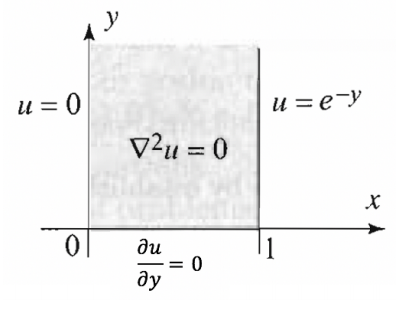
\includegraphics[width = .4\linewidth]{Prob3a.png}
			\end{figure}
			\\ 
			Notice the following boundary conditions:
			\[u(0,y) = 0 \qquad \pard{u}{y}(x,0) = 0 \qquad u(1,y) = e^{-y}\]
			We can let $u(x,y) = f(x)g(y)$ and $\lambda > 0$ to get the following:
			\[f''g = -fg'' \qqarrow \frac{f''}{f} = -\frac{g''}{g} = -\lambda \qquad f'' + \lambda f = 0 \qquad g'' - \lambda g = 0\]
			From our $x$-dependent ODE and its boundary condition $f(0) = 0$, we get the following:
			\[f(x) = c_2\sin\sqrt{\lambda}x\]
			From our $y$-dependent ODE and its boundary condition $g'(0) = 0$ along with the boundedness condition that $g(y)$ must be finite as $y \approches \infty$, we get the following:
			\[g(y) = d_1e^{-\sqrt{\lambda}y} \]
			Thus we get the following for $u(x,y)$:
			\[u(x,y) = A(y)\sin\sqrt{\lambda}xe^{-\sqrt{\lambda}y}\]
			Using the other boundary condition now gets us:
			\[A(y) = \frac{1}{\sin\sqrt{\lambda}e^{\left( -\sqrt{\lambda} + 1 \right)y}}\]
			\newpage
			% \item Use your solution to create a 3D plot of $u(x, y)$ with $y \in [0, 1]$. Your program should
			% integrate at least $\omega = [0, 50]$ for Fourier transforms. Be sure to include your program.
		\end{enumerate}
	\end{problem}

	% Exam 2 - Problem 5
	\begin{problem}{4}
		 Solve the nonhomogeneous heat equation
		 \[\pard{u}{t} = \nabla^2u + \sin(2x)\sin(3y), \qquad 0 < x < \pi, \quad 0 < y < \pi, \quad t > 0,\]
		 \[u(x,y,0) = \sin(4x)\sin(7y) \qquad u(x,0,t) = u(x,\pi,t) = u(0,y,t) = u(\pi,y,t) = 0\]
		 Let the following be true:
		 \[u(x,y,t) = f(x)g(y)h(t)\]
		 Using separation of variables, we get:
		 \[f'' = -\lambda f \qquad g'' = -\mu g \qquad h' + (\lambda + \mu)h = 0\]
		 Notice the following for the $x$ dependent equation, we get:
		 \[f_(x) = a_1\cos\sqrt{\lambda}x + a_2\sin\sqrt{\lambda}x\]
		 Now we apply the following boundary conditions, $f(0) = f(\pi) = 0$:
		 \[f(0) = a_1 = 0 \qquad f(\pi) = a_2\sin\sqrt{\lambda}\pi \qquad \lambda_m = m^2\]
		 Notice the following for the $y$ dependent equation, we get:
		 \[g(y) = b_1\cos\sqrt{\mu}y + b_2\sin\sqrt{\mu}y\]
		 Now we apply the following boundary conditions, $g(0) = g(\pi) = 0$:
		 \[g(0) = b_1 = 0 \qquad g(\pi) = b_2\sin\sqrt{\mu}\pi \qquad \mu_n = n^2\]
		 Notice the following for the $t$ dependent equation, we get:
		 \[h(t) = Ce^{-(\lambda + \mu)t}  \]
		 Thus we get the following:
		 \[u(x,y,t) = \sum_{m=1}^\infty \sum_{n=1}^\infty A_{mn}\sin(mx)\sin(ny)e^{-(\lambda + \mu)t} \]
		 Now notice the resubstitution into our original equation:
		 \[\sum_{m=1}^\infty \sum_{n=1}^\infty \left(\left(m^2 + n^2\right) - (\lambda + \mu)\right)A_{mn}e^{-(\lambda + \mu)t}\sin(mx)\sin(ny) = \sin(2x)\sin(3y)\]
	 	Thus, we get the following for $m \not= 2$ and $n \not= 3$:
		\[A_{mn} = 0\]
		Thus we get the following for $u(x,y,t)$:
		\[u(x,y,t) = A_{(2)(3)}\sin(2x)\sin(3y)e^{-(\lambda + \mu)t} \]
		 Now we can apply our initial condition and get:
		 \[u(x,y,0) = \sin(4x)\sin(7y) = A_{(2)(3)}\sin(2x)\sin(3y)\]
		 Thus we get the following for $A_{(2)(3)}$:
		 \[A_{(2)(3)} = \frac{4}{\pi^2}\int_{0}^\pi \int_{0}^\pi \sin(4x)\sin(7y)\sin(2x)\sin(3y)\,dx\,dy\]
	\end{problem}
	
	% Page 374 8.3.6
	\begin{problem}{5}
		Solve the nonhomogeneous partial differential equation:
		\[\pard{u}{t} = \pard{^2u}{x^2} + e^{-2t}\sin(5x), \qquad t > 0 \qtext{and} 0 < x < \pi,\]
		with initial and boundary conditions:
		\[u(x,0) = 0, \qquad u(0,t) = 1 \qtext{and} u(\pi,t) = 0\]
		We can begin by solving for the steady state problem ($t \approches \infty$):
		\[\frac{d^2u_E}{dx^2} = 0 \qtext{with} u_E(0) = 1 \qquad u_E(\pi) = 0\]
		Solving this, we get the following:
		\[u_E(x) = \frac{-x}{\pi} + 1\]
		Now we can resubstitute the following:
		\[v(x,t) = u(x,t) - u_E(x) \qquad \pard{v}{t} = \pard{^2v}{x^2} + e^{-2t}\sin(5x) \qquad v(0,t) = 0 \quad v(\pi) = 0 \quad v(x,0) = \frac{x}{\pi} - 1\]
		We now solved for $v(x,t)$'s eigenfunction and its solution:
		\[\phi_n(x) = \sin nx \qquad v(t) = \sum_{n=1}^{\infty} a_n(t)\sin nx\]
		Now we can resubstitute this into our original equation:
		\[\sum_{n=1}^{\infty} \frac{da_n(t)}{dt}\sin nx = -\sum_{n=1}^{\infty} n^2 a_n(t)\sin nx + e^{-2t}\sin(5x)\]
		Notice we get the following:
		\[\sum_{n=1}^{\infty} \left( \frac{da_n(t)}{dt} + n^2 a_n(t) \right)\sin nx = e^{-2t}\sin(5x)\]
		Solving for $a_n$ when $n \not = 5$:
		\[\frac{da_n(t)}{dt} + n^2 a_n(t) = 0 \qqarrow a_n(t) = a_n(0)e^{-n^2t}\]
		Solving for $a_n$ when $n = 5$:
		\[\frac{da_5(t)}{dt} + 25 a_5(t) = e^{-2t} \qqarrow a_5(t) = \frac{e^{-2t}}{23} + \left(a_5(0) - \frac{1}{23}\right)e^{-25t}\]
		Now we can use our initial condition to solve for $a_n(0)$:
		\[v(x,0) = \sum_{n=1}^{\infty} a_n(0)\sin nx =  \frac{x}{\pi} - 1 \qqarrow a_n(0) = \frac{2}{\pi}\int_{0}^{\pi} \left(\frac{x}{\pi} - 1\right)\sin nx\,dx = \frac{-2}{n\pi}\]
		Thus, we get the solution:
		\[u(x,t) = v(x,t) + u_E(x) = \sum_{n=1}^{\infty} a_n(t)\sin nx + \frac{-x}{\pi} + 1\]
	\end{problem}

	% Page 367 8.2.3
	\begin{problem}{6}
		Solve the nonhomogeneous two-dimensional heat equation with circularly symmetric time
		independent sources, boundary conditions, and initial conditions (inside a circle)

		\[\pard{u}{t} = \frac{k}{r}\pard{}{r}\left(r\pard{u}{r}\right) + Q(r)\]
		with
		\[u(r,0) = f(r) \qtext{and} u(a,t) = T.\]
		We can begin by solving for the steady state problem ($t \approches \infty$):
		\[\frac{k}{r}\frac{d}{dr}\left(r\frac{du_E}{dr}\right) + Q(r) = 0 \qqarrow  \frac{d}{dr}\left(r\frac{du_E}{dr}\right) = \frac{-rQ(r)}{k} \qqarrow \frac{du_E}{dr} = \frac{-1}{kr}\int rQ(r)\,dr\]
		Now we can solve for $u_E$:
		\[\int_a^r \frac{du_E}{dr} = u_E(r) - u_E(a) = \int_a^r \frac{-1}{kr}\int rQ(r)\,dr\,dr \qquad u_E(r) = \int_a^r \frac{-1}{kr}\int rQ(r)\,dr\,dr + T\]
		Now we can resubstitute the following:
		\[v(r,t) = u(r,t) - u_E(r) \qquad \pard{v}{t} = \frac{k}{r}\pard{}{r}\left(r\pard{v}{r} - r\pard{u_E}{r}\right) + Q(r) \qqarrow \pard{v}{t} = \frac{k}{r}\pard{}{r}\left(r\pard{v}{r}\right) \]
		with the following conditions:
		\[v(r,0) = f(r) - u_E(r) \qquad v(a,t) = 0\]
		We now solved for $v(r,t)$'s eigenfunction and eigenvalues and got the following:
		\[\phi_n(r) = c_1J_0\left(\sqrt{\lambda_n}r\right) \qqarrow \lambda_n = \left(\frac{z_n}{a}\right)^2  \]
		We now solved for $v(r,t)$ time dependent equation and got the following:
		\[h(t) = e^{-\lambda_n kt}\]
		Thus we get the following for $v(r,t)$:
		\[v(r,t) = \sum_{n=1}^\infty A_nJ_0\left(\sqrt{\lambda_n}t\right)e^{-\lambda_n kt} \]
		We now solve the following coefficients, using the initial condition:
		\[A_n = \frac{\int_0^a \left(f(r) - u_E(r)\right)J_0\left(\sqrt{\lambda_n}t\right)r\,dr }{\int_0^a J_0^2\left(\sqrt{\lambda_n}t\right)r\,dr}\]
		Thus we get the solution:
		\[u(r,t) = v(r,t) + u_E(r) = \sum_{n=1}^\infty A_nJ_0\left(\sqrt{\lambda_n}t\right)e^{-\lambda_n kt} + \int_a^r \frac{-1}{kr}\int rQ(r)\,dr\,dr + T\]
	\end{problem}

\end{document}
